\section{Trigonometric Functions}
We assume that the reader is already familiar with sines and cosines and will not repeat the well-known definitions here. But before we can do calculus with these things, we have to consider a mildly subtle point about what units we should  use to measure angles. When computing distance or speed, the absolute sizes of our units do not really matter; the meter and the foot are just conventions, we can just as well take one unit of length to be the distance from earth to the sun or the diameter of an atom. But trig functions are a bit different. A right angle is a right angle, and we cannot do anything without knowing how many units make a right angle. Traditionally we say ninety, because that makes a lot of computations come out cleanly -- a half, third, fifth, or sixth of a right angle is a whole number of degrees.\footnote{This was a big deal back in the days when all computations had to be done by hand! Also the sun moves a quarter of the the way around the zodiac in about 90 days -- i.e. roughly one degree per day, which was useful for astronomy.}

But there is another, equally standard approach, which works far better for our purposes. We will imagine all angles drawn at the center of a circle of radius ``one unit", and the measure of an angle is the length of the arc it spans. Since the circumference of our circle is $2\pi$, a right angle is one-quarter of the circumference, or $\pi/2$.  Since $r=1$, the area of our circle is $\pi$, and we can just as well say that an angle is measured as double the area of its wedge. This is known as measuring angles in \emph{radians}. From here forward, ``degrees" are banished to the dustbin of history! When measuring angles in radians, it can be useful to imagine walking counter-clockwise around a unit circle, starting at $(1,0)$; if we have gone distance $\theta$ along the arc, then we are at the point $(\cos(\theta), \sin(\theta))$. If $\theta < 0$, we are moving clockwise.
%add diagram for angle measurement

If we are going to combine calculus with trigonometry, our first order of business is to find the derivatives of trig functions. The derivative of $\sin(x)$ is
\[
\lim \frac{\sin(x+d_n)-\sin(x)}{d_n}
\]
Where $\lim d_n = 0$. What can we do with such an expression? It looks like the summation rule for sines is the thing to try here; we recall from high-school trigonometry that
\[
\sin(\alpha + \beta) = \sin(\alpha)\cos(\beta) + \sin(\beta)\cos(\alpha)
\]
Ideally we should prove this formula, but since it is so well-known we will give ourselves a bit of a break and just take it for granted. Applying  it to our problem yields
\[
\sin'(x) = \lim \frac{\sin(x)\cos(d_n) + \sin(d_n)\cos(x)-\sin(x)}{d_n}
\]
Believe it or not, this is progress! The factors $\sin(x)$ and $\cos(x)$ are constants which we can pull out of the limit if we break up the sum.  We get
\[
\sin'(x) = \sin(x)\lim \frac{\cos(d_n) - 1}{d_n} + \cos(x)\lim \frac{\sin(d_n)}{d_n}
\]
How would we evaluate such limits? We do not have a ``formula" for sines and cosines, which means we cannot get very far by algebraic manipulation alone; we need to reason about the geometric meaning of our equation. So we draw a diagram as in figure \ref{fig:sine}.

Taking one thing at a time, we will first attack $\lim \sin(d_n)/d_n$. The shaded area in the diagram is $d_n/2$. We will associate an angle with the area of a wedge (rather than with the length of an arc) because it is much easier to reason about areas: if one figure is completely inside another, we know that the interior figure has smaller area, even if we know nothing else about what these areas are. This suggests using our results about limits and inequalities; we will trap our challenging limit between two things we can calculate more easily.

We thus want to find the largest simple shape contained in the wedge, and the smallest simple shape that contains the wedge, where ``simple" means something whose area we know how to compute. In the diagram, we can see that there is a right triangle entirely inside the wedge; if we add the box to the right, we have a trapezoid which contains the wedge. Thus
\[
\frac{1}{2}\sin(d_n)\cos(d_n) < d_n/2 <  \frac{1}{2}\sin(d_n)\cos(d_n) + \sin(d_n)\left(1 - \cos(d_n)\right)
\]
A little algebraic simplification takes us to
\[
\sin(d_n)\cos(d_n) < d_n <   \sin(d_n)\left(2 - \cos(d_n)\right)
\]

\begin{figure}
\begin{center}
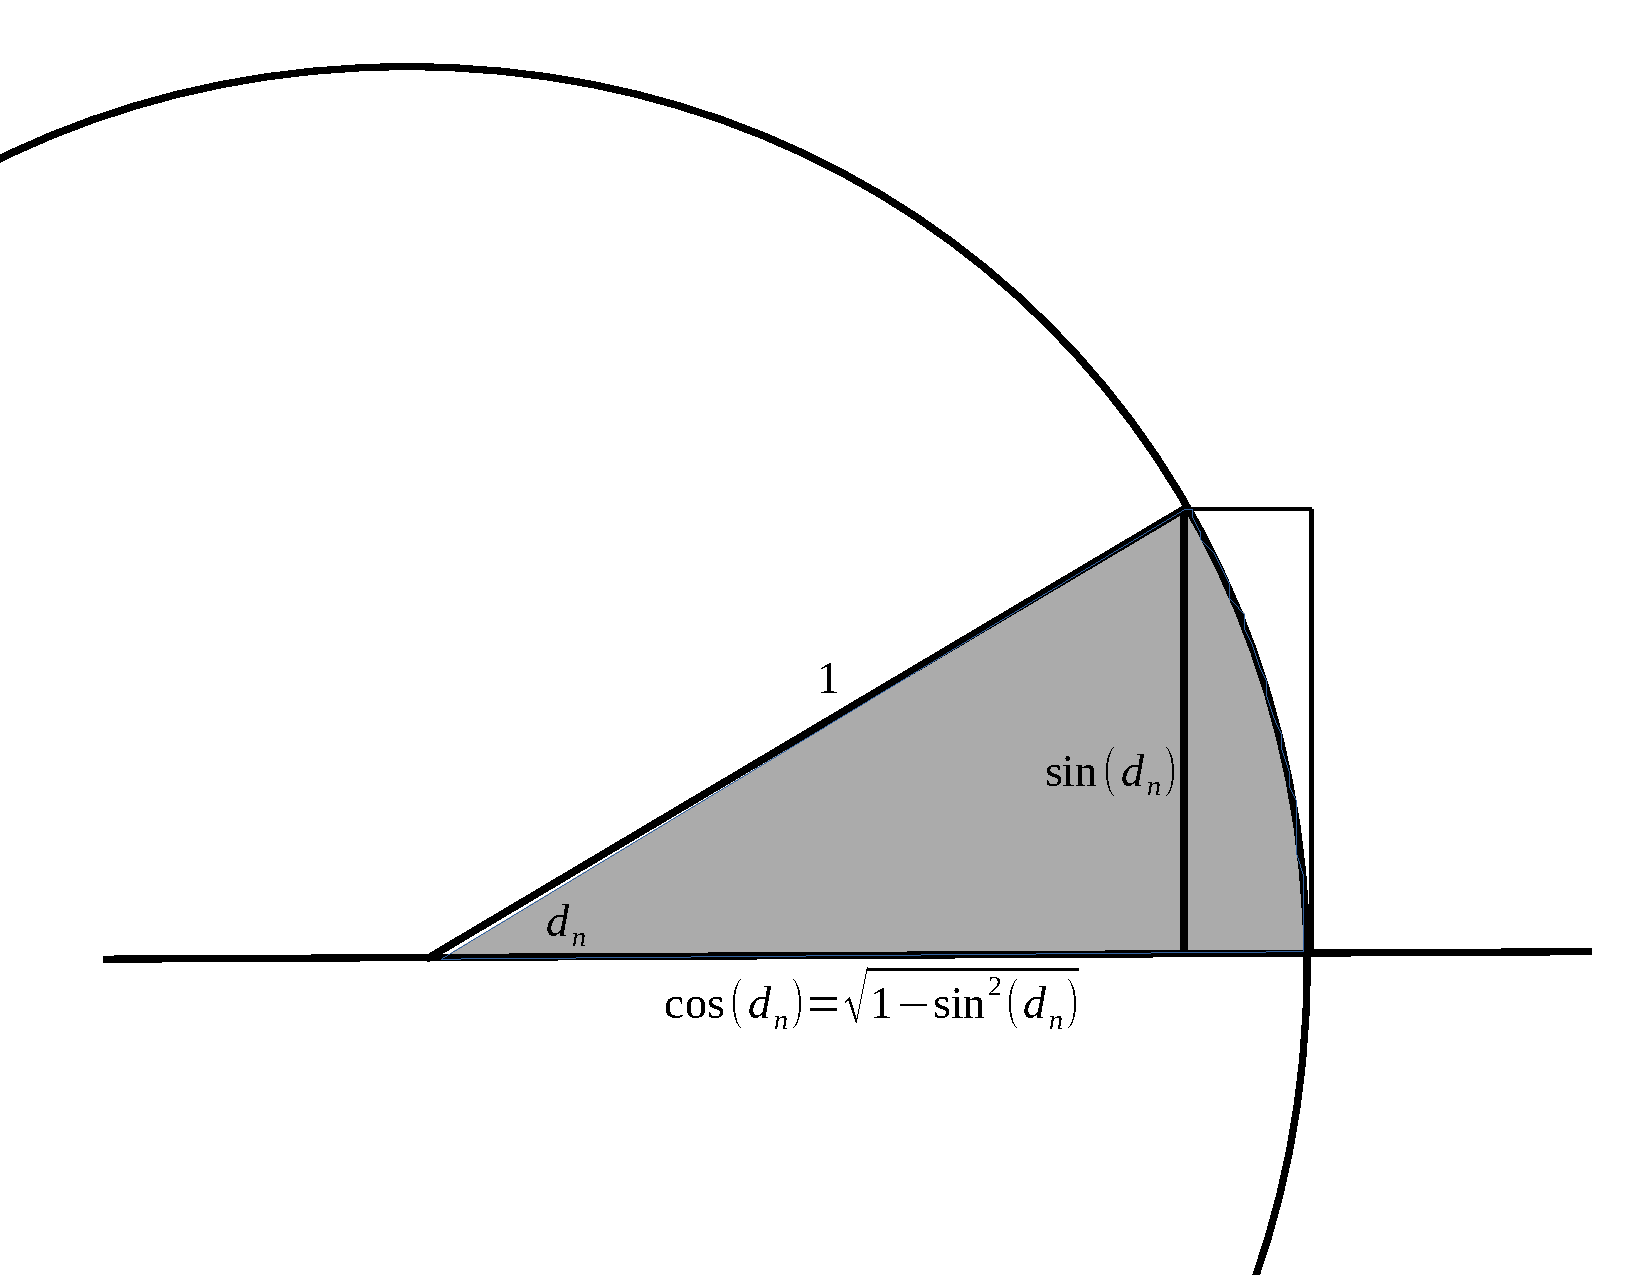
\includegraphics[scale=0.33]{trig}
\end{center}
\caption{Derivative of $\sin(x)$\label{fig:sine}}
\end{figure}


Dividing $\sin(d_n)$ into each term gives
\[
\frac{1}{\cos(d_n)} > \frac{\sin(d_n)}{d_n} >   \frac{1}{2 - \cos(d_n)}
\]
so as $d_n$ approaches zero, since $\cos(0)=1$ we have (assuming the cosine to be continuous)
\[
1 \geq \lim \frac{\sin(d_n)}{d_n} \geq   1\ .
\]

So far then
\[
\sin'(x) =  \sin(x)\lim \frac{\cos(d_n) - 1}{d_n} + \cos(x)
\]
Using the same kind of reasoning, we leave it to the reader to show that
\[
\lim \frac{\cos(d_n) - 1}{d_n} = 0
\]
thus establishing
\begin{thm}\label{thm:DerivOfSin}
\[
\sin'(x) = \cos(x)
\]  
\end{thm}

%Compare graphs of these functions, recall theorem about max derivative at zero

\subsection{Exercises}
Prove:
\begin{enumerate}
\item $\cos'(x) = -\sin(x)$
\item If $x$ is in degrees instead of radians, what is $\sin'(x)$?

%Make sure that other half of proof (left for reader) is not really too different.
\end{enumerate}


%\subsection{Series Expansion of Trig Functions}
%We noted above that we do not have an algebraic formula for $\sin(x)$. We did not need a formula to prove theorem \ref{thm:DerivOfSin}, but how would we actually evaluate something specific like $\sin(2\pi/7)$? If we carefully mark out the required distance around a large circle, we can see that it must be roughly $0.8$; any computer language or calculator will give us a more accurate value like $0.7818314824680297$, but such a number is not obtained by making measurements more carefully! It turns out that this is yet another case where limits are what we need; we will derive a sequence of algebraic expressions $a_n(x)$ whose limit is $\sin(x)$. Along the way we will find a sequence that converges to $\pi$; then we will, perhaps, be able to claim to understand what is usually just taken for granted, that $\pi = 3.1415926\cdots$.
%
%Is there, in fact, a purely geometric way to get the series expansions? Cannot find one.
%
%I think Spivak depends on integration to derive the series (or Taylor's theorem? and where will Taylor series fit in this book?). And is there a sequence-oriented way to get integrals? Yes; define the integral as the common value, if it exists, of a collection of sequences -- can we even link antidifferentiation? 
%
%Arc length -- eventually will define this as sum of short segments, so it will be possible to reason geometrically about lengths as well as areas.
%
%Deriving an expression for $\pi$ purely geometrically?


